\documentclass[tikz, border=1pt]{standalone}
\usepackage{tikz}
\usetikzlibrary{arrows.meta, positioning}
\usepackage{xcolor,colortbl}
% Define extra colors
\definecolor{darkgreen}{rgb}{0.0, 0.5, 0.0} % Define a darker green

\begin{document}

% \begin{figure}[h]
%     \centering

%     \begin{tikzpicture}[
%         claim/.style={rectangle, draw, rounded corners, align=center, text width=4cm, minimum height=1.5cm, fill=blue!20},
%         premise/.style={rectangle, draw, rounded corners, align=center, text width=4cm, minimum height=1.5cm, fill=yellow!50},
%         arrow/.style={-{Stealth}, thick},
%         support/.style={draw, -{Stealth}, thick, darkgreen},
%         attack/.style={draw, -{Stealth}, thick, red},
%         node distance=1cm and 1cm
%         ]

%         % Nodes
%         \node (claim1) [claim] {C1: l'adhésion de la Finlande à l'Otan devient un scénario de plus en plus crédible};
%         \node (premise1) [premise, right=of claim1] {P1: Un bouleversement de la politique extérieure de ce pays nordique qui a longtemps soigneusement évité la confrontation avec son voisin russe};
%         \node (claim2) [claim, below=of premise1] {C2: C'est un basculement historique de l'opinion publique finlandaise};
%         \node (claim3) [claim, below=of claim1] {C3: Au sein de la classe politique, le débat est ouvert et la question de la sacro-sainte neutralité finlandaise apparaît de plus en plus secondaire dans le contexte sécuritaire actuel};
%         \node (premise2) [premise, right=of claim2] {P2: Selon un sondage publié cette semaine, 62 \% de la population se dit favorable à rejoindre l'Otan};
%         \node (premise3) [premise, below=of claim2] {P3: Il y a deux semaines, une autre enquête avait pour la première fois donné une majorité absolue (53 \%) à cette adhésion à l'alliance militaire occidentale, soit un bond de près de 25 points, après l'invasion russe de l'Ukraine};
%         \node (premise4) [premise, below=of claim3] {P4: Dès le début de l'attaque menée par Vladimir Poutine, la Première ministre Sanna Marin avait annoncé qu'elle allait fournir des armes à l'Ukraine, du jamais vu pour ce pays nordique, militairement non aligné mais membre de l'Union européenne};

%         % Arrows with labels
%         \draw [support] (premise1) -- node[midway, above] {supports} (claim1);
%         \draw [support] (premise2) -- node[midway, above] {supports} (claim2);
%         \draw [support] (premise3) -- node[midway, above] {supports} (claim2);
%         \draw [support] (premise4) -- node[midway, right] {supports} (claim3);
%         \draw [support] (claim2) -- node[midway, right] {supports} (claim1);
%         \draw [support] (claim3) -- node[midway, right] {supports} (claim1);

%     \end{tikzpicture}
% \end{figure}

\begin{figure}
    \centering

    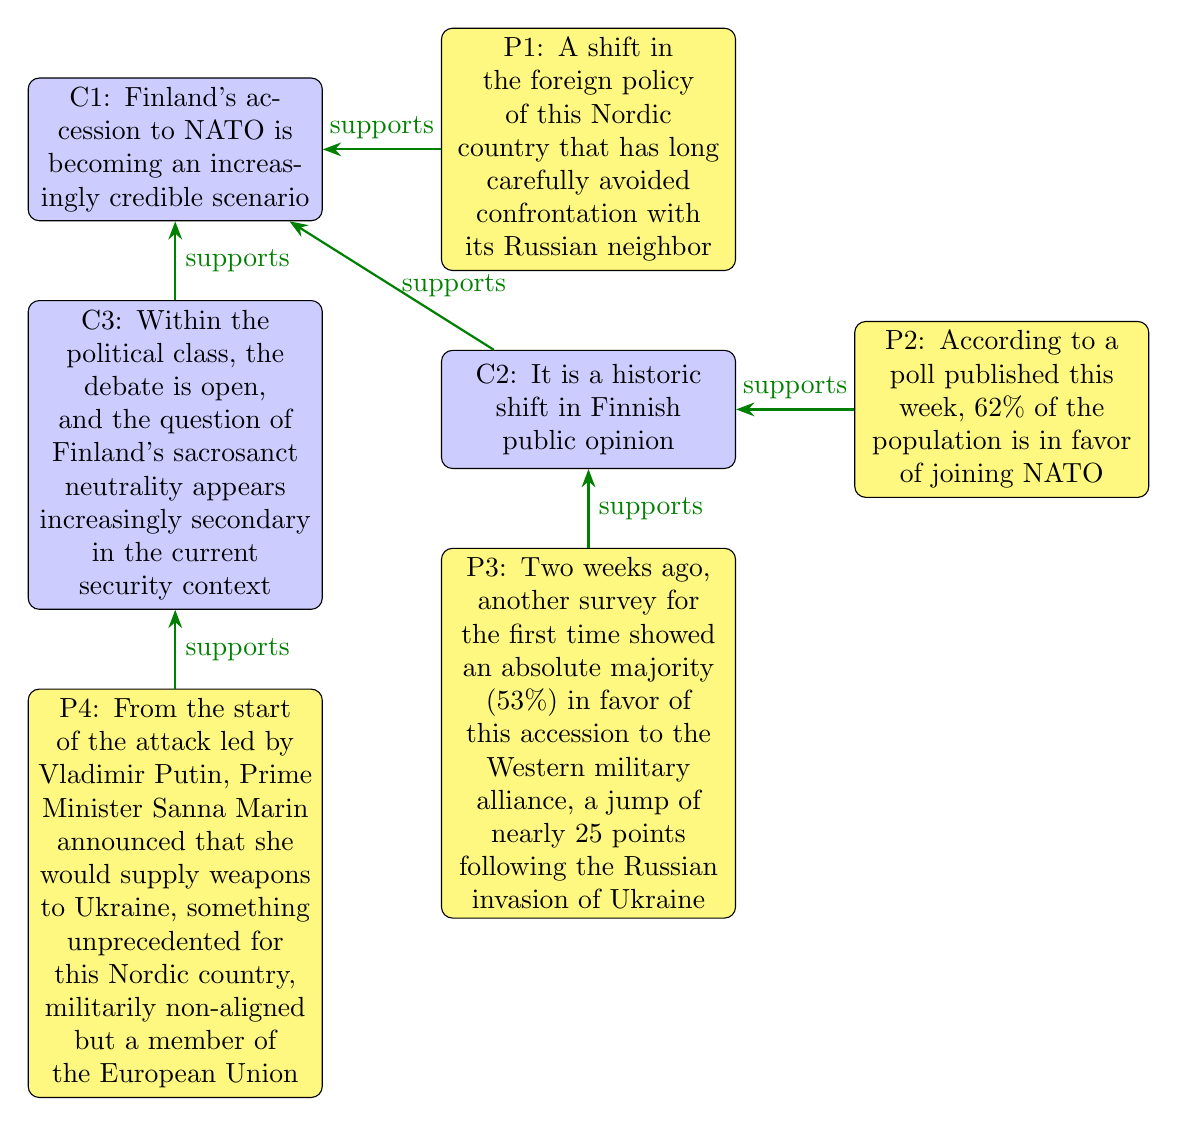
\begin{tikzpicture}[
        claim/.style={rectangle, draw, rounded corners, align=center, text width=3.5cm, minimum height=1.5cm, fill=blue!20},
        premise/.style={rectangle, draw, rounded corners, align=center, text width=3.5cm, minimum height=1.5cm, fill=yellow!50},
        arrow/.style={-{Stealth}, thick},
        support/.style={draw, -{Stealth}, thick, darkgreen},
        attack/.style={draw, -{Stealth}, thick, red},
        node distance=1cm and 1.5cm
        ]

        % Nodes
        \node (claim1) [claim] {C1: Finland's accession to NATO is becoming an increasingly credible scenario};
        \node (premise1) [premise, right=of claim1] {P1: A shift in the foreign policy of this Nordic country that has long carefully avoided confrontation with its Russian neighbor};
        \node (claim2) [claim, below=of premise1] {C2: It is a historic shift in Finnish public opinion};
        \node (claim3) [claim, below=of claim1] {C3: Within the political class, the debate is open, and the question of Finland's sacrosanct neutrality appears increasingly secondary in the current security context};
        \node (premise2) [premise, right=of claim2] {P2: According to a poll published this week, 62\% of the population is in favor of joining NATO};
        \node (premise3) [premise, below=of claim2] {P3: Two weeks ago, another survey for the first time showed an absolute majority (53\%) in favor of this accession to the Western military alliance, a jump of nearly 25 points following the Russian invasion of Ukraine};
        \node (premise4) [premise, below=of claim3] {P4: From the start of the attack led by Vladimir Putin, Prime Minister Sanna Marin announced that she would supply weapons to Ukraine, something unprecedented for this Nordic country, militarily non-aligned but a member of the European Union};

        % Arrows with labels
        \draw [support] (premise1) -- node[midway, above] {supports} (claim1);
        \draw [support] (premise2) -- node[midway, above] {supports} (claim2);
        \draw [support] (premise3) -- node[midway, right] {supports} (claim2);
        \draw [support] (premise4) -- node[midway, right] {supports} (claim3);
        \draw [support] (claim2) -- node[midway, right] {supports} (claim1);
        \draw [support] (claim3) -- node[midway, right] {supports} (claim1);

    \end{tikzpicture}
    % \caption{Argumentation structure for the Example \ref{ex:france24}}
    \label{fig:france24}
\end{figure}

\end{document}
